
\documentclass[conference,a4paper]{IEEEtran}

% ==========================================
% CẤU HÌNH IEEE TIẾNG VIỆT
% Compiler: XeLaTeX
% ==========================================

\usepackage{fontspec}
\usepackage[vietnamese]{babel}
\setmainfont{TeX Gyre Termes}

\usepackage{amsmath,amssymb}
\usepackage{graphicx}
\usepackage{booktabs}
\usepackage{tabularx}
\usepackage{array}
\usepackage{caption}
\usepackage{url}
\usepackage{cite}
\usepackage{microtype}

\graphicspath{{images/}{reports/figures/}}

\captionsetup{
    font=footnotesize,
    labelfont=bf
}

\renewcommand{\abstractname}{Tóm tắt}
\renewcommand{\IEEEkeywordsname}{Từ khóa}
\renewcommand{\refname}{Tài liệu tham khảo}

% ==========================================
% KHUNG HÌNH GIỮ CHỖ
% Có thể dùng cho các phần sau
% ==========================================

\newcommand{\imageplaceholder}[2]{
    \begin{figure}[!t]
        \centering
        \fbox{
            \parbox[c][3cm][c]
            {0.92\columnwidth}{
                \centering
                \footnotesize
                \texttt{\detokenize{#1}}
            }
        }
        \caption{#2}
    \end{figure}
}

\begin{document}

% ==========================================
% TIÊU ĐỀ BÀI BÁO
% ==========================================

\title{
PHÂN TÍCH HÀNH VI CHIẾM DỤNG
VÀ DỰ BÁO NHU CẦU SẠC NHẰM
NÂNG CAO HIỆU SUẤT VẬN HÀNH
MẠNG LƯỚI TRẠM SẠC XE ĐIỆN
CÔNG CỘNG
}

% ==========================================
% THÔNG TIN NHÓM
% ==========================================

\author{
\IEEEauthorblockN{
Nguyễn Mai Kỳ,
Trương Như Khải,
Hồ Thị Thùy Dung,
Nguyễn Thị Lam Giang
}
\IEEEauthorblockA{
Khoa Hệ thống Thông tin\\
Trường Đại học Công nghệ Thông tin\\
Đại học Quốc gia TP. Hồ Chí Minh\\
TP. Hồ Chí Minh, Việt Nam\\
IS403 -- Phân tích dữ liệu kinh doanh
}
}

\maketitle

% ==========================================
% TÓM TẮT
% ==========================================

\begin{abstract}

Sự phát triển của phương tiện giao thông điện
đặt ra yêu cầu nâng cao hiệu quả khai thác
hạ tầng sạc công cộng, đặc biệt trong bối cảnh
thời gian phương tiện chiếm giữ cổng sạc
không hoàn toàn tương ứng với thời gian
truyền điện thực tế.

Nghiên cứu này xây dựng một quy trình
phân tích dữ liệu kinh doanh nhằm đánh giá
hành vi sử dụng, mức độ chiếm dụng nhàn rỗi,
hiệu suất vận hành và nhu cầu sạc
của mạng lưới trạm sạc công cộng
tại Palo Alto, California, Hoa Kỳ.

Bộ dữ liệu gốc gồm 259.415 phiên sạc,
chủ yếu thuộc giai đoạn 2011--2020.
Quy trình nghiên cứu bao gồm năm nhiệm vụ:
kiểm soát chất lượng dữ liệu;
phân nhóm hành vi bằng K-Means và DBSCAN;
phân tích sự khác biệt trước và sau
thay đổi chính sách giá;
xếp hạng hiệu suất trạm bằng Entropy--TOPSIS;
và dự báo nhu cầu, mức độ chiếm dụng
bằng các mô hình học máy,
trong đó có XGBoost.

Kết quả tiền xử lý xác định 259.356 phiên
đạt điều kiện hợp lệ của NV1.
Phân tích K-Means trên 258.720 phiên
nhận diện bốn nhóm hành vi,
trong đó nhóm chiếm dụng nhàn rỗi kéo dài
chiếm 2,67\% số phiên.
Đánh giá TOPSIS được thực hiện trên
33 trạm theo sáu tiêu chí vận hành.

Các kết quả phân tích cung cấp cơ sở
để xem xét chính sách quản lý thời gian
nhàn rỗi, đánh giá sự khác biệt giữa các trạm
và hỗ trợ quyết định vận hành.
Các kết quả dự báo được đánh giá
theo phân hoạch thời gian và đối chiếu
với các mô hình cơ sở.

\end{abstract}

\begin{IEEEkeywords}
Xe điện, trạm sạc công cộng,
chiếm dụng nhàn rỗi, Idle Time,
K-Means, DBSCAN, Mann--Whitney U,
TOPSIS, XGBoost, dự báo nhu cầu.
\end{IEEEkeywords}


% ==========================================
% I. GIỚI THIỆU
% ==========================================

\section{GIỚI THIỆU}

\subsection{Bối cảnh nghiên cứu}

Trong những năm gần đây,
phương tiện giao thông điện ngày càng
được quan tâm như một giải pháp
hướng đến giảm phát thải trong
lĩnh vực giao thông vận tải.
Cùng với sự gia tăng phương tiện điện,
nhu cầu phát triển hạ tầng sạc
công cộng cũng trở nên quan trọng.

Tuy nhiên, hiệu quả vận hành mạng lưới
trạm sạc không chỉ phụ thuộc vào
số lượng trạm hoặc cổng sạc được lắp đặt.
Khả năng khai thác hạ tầng
còn chịu ảnh hưởng bởi vị trí,
thời gian phát sinh nhu cầu,
thời lượng kết nối và hành vi sử dụng
của người điều khiển phương tiện.

Bayram và cộng sự \cite{bayram2023}
đã phân tích gần 12.000 phiên sạc
từ 595 cổng sạc AC công cộng
tại Vương quốc Anh.
Nghiên cứu cho thấy hoạt động sử dụng
trạm có sự khác biệt đáng kể
theo thời điểm, loại cổng
và thời gian phương tiện lưu trú.
Việc phân tích các đặc trưng vận hành
giúp cung cấp thông tin cho
quy hoạch và quản lý hạ tầng sạc.

Trong thực tế, một trạm có số lượng
cổng sạc lớn chưa chắc đạt hiệu suất
phục vụ tương ứng.
Tương tự, một trạm có tổng thời gian
kết nối cao chưa chắc cung cấp
lượng điện năng lớn,
bởi phương tiện có thể tiếp tục
chiếm giữ cổng sau khi kết thúc
quá trình truyền điện.

Do đó, phân tích hiệu quả khai thác
hạ tầng sạc cần tiếp cận từ nhiều
góc độ, bao gồm nhu cầu sử dụng,
thời lượng sạc thực tế,
thời gian chiếm dụng nhàn rỗi
và sự phân bố hoạt động theo thời gian.

\subsection{Vấn đề chiếm dụng nhàn rỗi}

Đối với một phiên sạc,
tổng thời gian phương tiện kết nối
với cổng sạc thường bao gồm
thời gian truyền điện thực tế
và khoảng thời gian phương tiện
tiếp tục giữ cổng nhưng không
nhận thêm điện năng.

Khoảng thời gian thứ hai được gọi là
\textit{Idle Time} hoặc
\textit{Overstay Time}.
Đây là một chỉ tiêu quan trọng
trong đánh giá hành vi sử dụng
trạm sạc công cộng.

Khi phương tiện vẫn chiếm giữ cổng
sau khi kết thúc sạc,
cổng đó chưa thể phục vụ
một phương tiện khác,
mặc dù hoạt động truyền điện
không còn tiếp diễn.
Điều này có thể làm giảm
khả năng phục vụ thực tế,
đặc biệt tại những địa điểm
có nhu cầu sử dụng cao.

Theo Bayram và cộng sự
\cite{bayram2023},
thời gian chiếm dụng sau sạc
có sự khác biệt giữa các loại
cổng và bối cảnh sử dụng.
Vì vậy, chỉ thống kê số phiên
hoặc điện năng cung cấp
chưa đủ để phản ánh
đặc điểm vận hành của hạ tầng.

Trong nghiên cứu này,
thời gian nhàn rỗi của phiên $i$
được xác định bằng:

\begin{equation}
T_{\mathrm{idle},i}
=
T_{\mathrm{total},i}
-
T_{\mathrm{charge},i}.
\label{eq:idle_time}
\end{equation}

Trong đó,
$T_{\mathrm{total},i}$ là tổng thời gian
kết nối và $T_{\mathrm{charge},i}$
là thời gian sạc thực tế.

Tỷ lệ thời gian nhàn rỗi
của phiên sạc được xác định:

\begin{equation}
R_{\mathrm{idle},i}
=
\frac{T_{\mathrm{idle},i}}
{T_{\mathrm{total},i}},
\quad T_{\mathrm{total},i}>0.
\label{eq:idle_ratio}
\end{equation}

Chỉ số Idle Time phản ánh
thời lượng nhàn rỗi tuyệt đối,
trong khi Idle Ratio cho phép
so sánh mức độ chiếm dụng
giữa những phiên có
thời gian kết nối khác nhau.

Hai chỉ số này tạo cơ sở
để nhận diện những nhóm hành vi
cần được quan tâm trong
công tác quản lý và vận hành
mạng lưới trạm sạc.

% ==========================================
% CHỖ CHÈN HÌNH TÙY CHỌN 1
%
% ---<Hinh minh hoa Idle Time va Charging Time>---
%
% Không bắt buộc giữ hình này vì hai
% công thức phía trên đã giải thích khái niệm.
%
% Nếu muốn dùng, bỏ dấu % ở các dòng dưới.
%
% \begin{figure}[!t]
%     \centering
%     \fbox{
%         \parbox[c][2.5cm][c]
%         {0.92\columnwidth}{
%             \centering
%             ---<Hinh Charging Time va Idle Time>---
%         }
%     }
%     \caption{Cấu trúc thời gian
%     của một phiên sạc xe điện.}
%     \label{fig:idle_explanation}
% \end{figure}
% ==========================================


\subsection{Mục tiêu và câu hỏi nghiên cứu}

Mục tiêu tổng quát của đề tài
là ứng dụng các phương pháp
phân tích dữ liệu kinh doanh
để nghiên cứu hành vi sử dụng,
mức độ chiếm dụng nhàn rỗi
và hiệu suất vận hành
mạng lưới trạm sạc xe điện công cộng.

Nghiên cứu sử dụng dữ liệu
các phiên sạc tại Palo Alto,
California, nhằm kết hợp
phân tích thống kê,
học máy và xếp hạng đa tiêu chí
trong một quy trình thống nhất.

Các câu hỏi nghiên cứu chính gồm:

\begin{enumerate}
\item
Hành vi sạc và chiếm dụng nhàn rỗi
có những đặc điểm nào?
Có thể nhận diện các nhóm
phiên sạc khác nhau bằng phân cụm
hay không?

\item
Các chỉ tiêu hành vi sử dụng trạm
khác nhau như thế nào giữa
giai đoạn trước và sau
thay đổi chính sách giá
ngày 01/08/2017?

\item
Hiệu suất vận hành giữa các trạm
có sự khác biệt ra sao
khi đánh giá đồng thời
nhiều tiêu chí?

\item
Có thể khai thác chuỗi dữ liệu
lịch sử để dự báo nhu cầu
và mức độ chiếm dụng
trong các khung thời gian
15 phút hay không?
\end{enumerate}

Để trả lời các câu hỏi trên,
đề tài triển khai năm nhiệm vụ.

NV1 thực hiện kiểm soát chất lượng,
tiền xử lý và xây dựng đặc trưng
dữ liệu phiên sạc.

NV2 sử dụng K-Means và DBSCAN
nhằm nhận diện các nhóm hành vi
sử dụng hạ tầng.

NV3 phân tích sự khác biệt
trước và sau thay đổi chính sách
bằng các phương pháp thống kê
và kiểm định phi tham số.

NV4 sử dụng TOPSIS kết hợp
trọng số Entropy và trọng số đều
để đánh giá, xếp hạng hiệu suất
của các trạm sạc.

NV5 xây dựng bài toán
dự báo chuỗi thời gian,
đối chiếu các mô hình cơ sở
với những thuật toán học máy,
trong đó có XGBoost.

Kết quả của năm nhiệm vụ được
tổng hợp thành tầng
hỗ trợ quyết định vận hành
(\textit{Decision Layer}),
phục vụ việc xem xét
quản lý thời gian nhàn rỗi,
đánh giá hiệu suất trạm
và phân bổ nguồn lực.

\subsection{Phạm vi và đóng góp nghiên cứu}

Nghiên cứu sử dụng dữ liệu
giao dịch sạc xe điện công cộng
tại thành phố Palo Alto,
bang California, Hoa Kỳ.
Bộ dữ liệu gốc gồm 259.415 phiên sạc
trong giai đoạn từ tháng 7/2011
đến đầu tháng 1/2021,
trong đó phần phân tích theo năm
tập trung chủ yếu vào 2011--2020.

Đối tượng phân tích bao gồm
phiên sạc, người dùng,
trạm sạc và các nhóm vị trí.
Những thuộc tính trọng tâm
là thời điểm bắt đầu và kết thúc,
tổng thời gian kết nối,
thời gian truyền điện,
điện năng tiêu thụ
và thông tin định danh trạm.

Đóng góp thứ nhất của nghiên cứu
là xây dựng quy trình phân tích
có kiểm soát chất lượng và đối soát
giữa các nhiệm vụ,
hạn chế việc sử dụng các tập dữ liệu
khác nhau mà không ghi rõ
điều kiện lọc.

Đóng góp thứ hai là kết hợp
nhiều phương pháp phân tích
trên các cấp độ khác nhau:
cấp phiên để phân nhóm hành vi,
cấp người dùng để xem xét
thay đổi cơ cấu,
cấp trạm để đánh giá hiệu suất
và cấp thời gian để dự báo nhu cầu.

Đóng góp thứ ba là chuyển hóa
các phát hiện định lượng
thành cơ sở thông tin hỗ trợ
quyết định vận hành,
thay vì chỉ dừng ở việc
so sánh các thuật toán.

Nghiên cứu có một số giới hạn.
Dữ liệu chỉ thuộc mạng lưới
tại Palo Alto,
nên không thể mặc định kết quả
đại diện cho mọi hệ thống sạc.

Bên cạnh đó,
việc so sánh hai giai đoạn
trước và sau chính sách
chỉ cho thấy sự khác biệt
quan sát được trong dữ liệu.
Những khác biệt này chưa đủ
để khẳng định quan hệ nhân quả
nếu không có thiết kế nhận dạng
phù hợp.

Đối với bài toán dự báo,
kết quả được đánh giá
trong bối cảnh dữ liệu lịch sử
và các điều kiện thực nghiệm
đã xác định.

% ==========================================
% II. NGHIÊN CỨU LIÊN QUAN
% ==========================================

\section{NGHIÊN CỨU LIÊN QUAN}

Các nghiên cứu về hạ tầng sạc
xe điện đã tiếp cận bài toán vận hành
theo nhiều hướng,
bao gồm mô tả hành vi sử dụng,
phân nhóm các mẫu sạc,
phân tích phản ứng trước chính sách giá
và dự báo trạng thái chiếm dụng.

Trong phạm vi đề tài,
bốn công trình được lựa chọn
làm cơ sở nghiên cứu chính.
Những công trình này cung cấp
định hướng về biến phân tích,
phương pháp thực nghiệm
và cách đánh giá kết quả,
đồng thời làm rõ những giới hạn
cần chú ý khi diễn giải
các phát hiện của nhóm.

\subsection{Phân tích thống kê hành vi
sử dụng trạm sạc}

Bayram và cộng sự \cite{bayram2023}
thực hiện nghiên cứu
``Statistical Characterization
of Public AC EV Chargers in the U.K.'',
được công bố trên IEEE Access
năm 2023.

Nghiên cứu khảo sát gần 12.000
phiên sạc được thu thập
từ 595 cổng sạc AC công cộng
tại Vương quốc Anh
trong khoảng tháng 4
đến tháng 7/2022.
Các cổng được khảo sát
thuộc hai mức công suất
7 kW và 22 kW.

Mục tiêu của công trình là
mô tả những đặc điểm
quan trọng của hoạt động sạc,
bao gồm mức độ sử dụng hạ tầng,
thời điểm phương tiện đến
và rời khỏi trạm,
thời lượng kết nối,
điện năng cung cấp
và thời gian chiếm dụng sau sạc.

Về phương pháp,
nhóm tác giả sử dụng
phân tích thống kê mô tả,
phân tích phân phối,
phân nhóm hành vi theo thời điểm
và đánh giá sự khác biệt
giữa loại cổng sạc,
ngày thường và cuối tuần.
Ngoài ra, nghiên cứu khảo sát
những yếu tố liên quan đến
thời gian chiếm dụng nhàn rỗi.

Kết quả cho thấy
hoạt động sử dụng trạm
không đồng đều giữa các địa điểm
và loại cổng.
Đặc biệt, thời gian phương tiện
tiếp tục kết nối sau quá trình sạc
có sự khác biệt đáng kể
giữa các nhóm cổng sạc,
cho thấy cần đánh giá
thời gian nhàn rỗi riêng
với thời gian truyền điện.

Nghiên cứu cũng phân tích
khả năng khai thác sự linh hoạt
trong thời gian kết nối
để hỗ trợ điều phối hoạt động sạc.
Những kết quả này cho thấy
dữ liệu phiên sạc không chỉ
phục vụ thống kê sản lượng,
mà còn có giá trị
đối với quản lý hạ tầng.

Tuy nhiên, phạm vi dữ liệu
thuộc mạng lưới tại Vương quốc Anh,
trong một giai đoạn quan sát
tương đối ngắn,
nên các đặc điểm thu được
có thể phụ thuộc vào
bối cảnh sử dụng cụ thể.

Đối với đề tài IS403,
công trình cung cấp
cơ sở phân biệt
tổng thời gian kết nối,
thời gian sạc thực tế
và thời gian chiếm dụng nhàn rỗi.

Hai chỉ số Idle Time
và Idle Ratio được sử dụng
để lượng hóa mức độ chiếm dụng
ở cấp phiên và hỗ trợ
phân tích hành vi tại NV1,
NV2 và hiệu suất trạm tại NV4.

\subsection{Phân cụm hành vi sử dụng
hạ tầng sạc}

Straka và Buzna \cite{straka2019}
công bố công trình
``Clustering Algorithms Applied
to Usage Related Segments
of Electric Vehicle Charging Stations''
trên Transportation Research Procedia
năm 2019.

Nghiên cứu tập trung
vào việc nhận diện những mẫu
sử dụng trạm sạc khác nhau
từ dữ liệu giao dịch,
qua đó hỗ trợ mô tả
các phân khúc sử dụng hạ tầng.

Thay vì giả định rằng
toàn bộ các phiên sạc
có cùng đặc điểm,
nhóm tác giả áp dụng
các phương pháp học không giám sát
để tìm kiếm cấu trúc tiềm ẩn
trong dữ liệu.

Ba phương pháp được khảo sát
gồm K-Means, DBSCAN
và phân cụm phân cấp kết tụ
(\textit{Agglomerative Clustering}).

K-Means tổ chức dữ liệu
thành các nhóm dựa trên
khoảng cách tới tâm cụm.
Trong khi đó,
DBSCAN hình thành cụm
từ mật độ quan sát
và cho phép tách riêng
những điểm không thuộc
vùng mật độ đủ lớn.

Việc đối chiếu các phương pháp
giúp đánh giá liệu
các nhóm sử dụng
có cấu trúc tập trung rõ rệt
hay tồn tại các quan sát
khó được đại diện bằng
những tâm cụm cố định.

Công trình cho thấy
phân cụm có thể hỗ trợ
nhận diện những phân khúc
liên quan đến cách sử dụng trạm.
Kết quả mang ý nghĩa
đối với quy hoạch
và phát triển hạ tầng,
bởi các nhóm người dùng
hoặc phiên sạc khác nhau
có thể tạo ra yêu cầu
vận hành không giống nhau.

Hạn chế cần lưu ý là
kết quả phân nhóm chịu ảnh hưởng
của bộ đặc trưng,
cách chuẩn hóa
và lựa chọn tham số thuật toán.
Các nhãn cụm không có
ý nghĩa nghiệp vụ cố định
nếu chưa được diễn giải
bằng những thuộc tính quan sát.

Kế thừa hướng tiếp cận này,
NV2 áp dụng K-Means và DBSCAN
trên các đặc trưng hành vi
được xây dựng từ dữ liệu
phiên sạc Palo Alto.

Nghiên cứu lựa chọn số cụm
dựa trên nhiều chỉ số,
bao gồm Silhouette,
Davies--Bouldin và WCSS;
đồng thời kiểm tra độ ổn định
bằng cách chia mẫu.

Điểm khác biệt là
các cụm trong đề tài
được diễn giải trực tiếp
theo thời gian sạc,
điện năng tiêu thụ
và mức độ chiếm dụng nhàn rỗi,
phù hợp với mục tiêu
đánh giá hiệu quả vận hành
ở cấp phiên sạc.

\subsection{Phân tích tác động
của chính sách giá}

Luo và Wang \cite{luowang2025}
nghiên cứu sự thay đổi
hành vi sạc xe điện
trong công trình
``The Impacts of Rate Surge
on Electric Vehicle Charging Behaviors:
Evidence from California'',
công bố năm 2025.

Nghiên cứu khai thác
bối cảnh chính sách giá
tại Palo Alto, California,
nơi dịch vụ sạc chuyển
từ miễn phí sang cơ chế
thu phí năng lượng
và phí đỗ xe sau sạc.

Từ ngày 01/08/2017,
mức thu phí năng lượng
được áp dụng là
0,23 USD/kWh,
cùng khoản phí
2 USD/giờ đối với
thời gian đỗ sau sạc
theo cơ chế của chính sách.

Điểm quan trọng của nghiên cứu
là sử dụng dữ liệu
ở cấp phiên sạc,
qua đó quan sát được
thời lượng, điện năng
và đặc điểm sử dụng trạm
trước và sau
thời điểm thay đổi giá.

Về phương pháp,
nhóm tác giả sử dụng
thiết kế hồi quy gián đoạn
theo thời gian
(\textit{Regression Discontinuity
in Time} -- RDiT).

Thiết kế này tập trung
vào biến động gần mốc
chính sách có hiệu lực,
đồng thời xem xét
những yếu tố có thể ảnh hưởng
đến hành vi sử dụng.

Theo kết quả được công bố,
số phiên sạc giảm khoảng
32,2\% sau thay đổi chính sách.
Điện năng trung bình mỗi phiên
giảm 20,5\%,
trong khi thời gian đỗ
không thực hiện sạc
giảm khoảng 72,3\%.

Những tỷ lệ này là
kết quả ước lượng
từ thiết kế nghiên cứu
của Luo và Wang,
không phải số liệu
được nhóm IS403 tính
bằng cách lấy chênh lệch
trung bình hai giai đoạn.

Công trình cũng nhấn mạnh
sự cần thiết phải phân biệt
thay đổi hành vi của
người dùng hiện hữu
với sự thay đổi thành phần
người sử dụng trạm.

Một biến động được ghi nhận
ở toàn mạng lưới
có thể đồng thời phản ánh
sự điều chỉnh của các cá nhân
và việc một số người
ngừng hoặc bắt đầu sử dụng dịch vụ.

Đối với IS403,
nghiên cứu của Luo và Wang
cung cấp cơ sở lựa chọn
mốc ngày 01/08/2017
và các chỉ tiêu hành vi
cần đối chiếu trong NV3.

Tuy nhiên, đề tài hiện tại
không tái triển khai
thiết kế RDiT của nghiên cứu gốc.
Thay vào đó, nhóm sử dụng
thống kê mô tả,
phân khúc người dùng,
kiểm định Mann--Whitney U,
Cliff's Delta
và bootstrap theo User ID.

Vì vậy, kết quả NV3
chỉ được diễn giải
như sự khác biệt quan sát được
giữa hai giai đoạn,
không khẳng định
quan hệ nhân quả
giữa chính sách và hành vi.

\subsection{Dự báo mức độ chiếm dụng
trạm sạc bằng học máy}

Ostermann và cộng sự
\cite{ostermann2022}
công bố nghiên cứu
``Forecasting Charging Point Occupancy
Using Supervised Learning Algorithms''
trên tạp chí Energies
năm 2022.

Nghiên cứu sử dụng
dữ liệu Adaptive Charging Network
(ACN) tại hai địa điểm
ở California,
bao gồm một địa điểm
phục vụ công cộng
và một địa điểm phục vụ
nhu cầu tại nơi làm việc.

Bài toán được chia thành
hai hướng dự báo.

Hướng thứ nhất là
xác định trạng thái
có hoặc không có phương tiện
chiếm dụng tại từng cổng sạc.

Hướng thứ hai là
dự báo số cổng bị chiếm dụng
trong toàn bộ địa điểm
tại một thời điểm.

Để thực hiện,
nhóm tác giả chuyển dữ liệu
phiên sạc thành chuỗi thời gian
với độ phân giải 15 phút.

Các biến đầu vào
bao gồm thông tin lịch
và trạng thái chiếm dụng
trong quá khứ,
nhằm khai thác tính chu kỳ
của hoạt động sử dụng trạm.

Các mô hình được khảo sát
gồm hồi quy tuyến tính
hoặc logistic,
K-Nearest Neighbors,
Random Forest và XGBoost,
tùy theo bài toán
hồi quy hoặc phân loại.

Hiệu quả dự báo
được đối chiếu bằng
các thước đo phù hợp
và so sánh với những
phương pháp cơ sở
dựa trên lịch sử sử dụng.

Kết quả cho thấy
khả năng dự báo phụ thuộc
đáng kể vào đặc điểm
của từng địa điểm và cổng sạc.
Thông tin chiếm dụng trong quá khứ
có giá trị đối với
việc dự báo trạng thái tiếp theo.

Tuy nhiên, các phương pháp
học máy phức tạp
không nhất thiết vượt trội
trong mọi trường hợp,
đặc biệt khi chuỗi dữ liệu
có mức sử dụng thấp
hoặc biến động mạnh.

Điểm hạn chế là
công trình khảo sát
những địa điểm cụ thể
với dữ liệu và điều kiện
vận hành khác Palo Alto.
Kết quả do đó không thể
chuyển trực tiếp thành
độ chính xác dự báo
của bộ dữ liệu IS403.

Đối với NV5,
nghiên cứu được kế thừa
ở cách xây dựng chuỗi 15 phút,
sử dụng đặc trưng thời gian,
biến trễ và tổ chức
mô hình đối chứng.

Đề tài đồng thời
tổ chức phân hoạch dữ liệu
theo thứ tự thời gian
để tránh rò rỉ
thông tin tương lai.

XGBoost được so sánh
với các phương pháp dự báo
dựa trên lịch sử
và các mô hình học máy khác,
nhằm đánh giá hiệu quả
trên dữ liệu ngoài mẫu.

\subsection{Tổng hợp các nghiên cứu
và khoảng trống nghiên cứu}

Bốn nghiên cứu trên
cung cấp những góc nhìn
bổ sung cho bài toán
vận hành hạ tầng sạc
xe điện công cộng.

Bayram và cộng sự
tập trung vào thống kê
hành vi sử dụng,
đặc biệt thời gian kết nối
và chiếm dụng sau sạc.

Straka và Buzna
khai thác khả năng
phân cụm để nhận diện
các nhóm sử dụng hạ tầng.

Luo và Wang
nghiên cứu phản ứng
của người dùng
trước thay đổi chính sách giá.

Ostermann và cộng sự
tập trung vào dự báo
trạng thái và số lượng
cổng sạc bị chiếm dụng.

Bảng~\ref{tab:related_work}
tóm tắt phương pháp
và nội dung được kế thừa
trong đề tài IS403.

% ==========================================
% BẢNG II.1 - NGHIÊN CỨU LIÊN QUAN
% Bảng trải ngang hai cột
% ==========================================


% Bảng nghiên cứu liên quan - bản rút gọn một cột
\begin{table}[!t]
\centering
\caption{Tổng hợp nghiên cứu liên quan}
\label{tab:related_work}

\scriptsize
\setlength{\tabcolsep}{3pt}
\renewcommand{\arraystretch}{1.05}

\begin{tabularx}{\columnwidth}{
@{}p{1.65cm} X p{0.65cm}@{}
}
\toprule
\textbf{Nghiên cứu} &
\textbf{Nội dung kế thừa} &
\textbf{NV}\\
\midrule

Bayram và cs. (2023) \cite{bayram2023}
& Idle Time, Idle Ratio và hành vi chiếm dụng.
& 1,2,4\\

Straka và Buzna (2019) \cite{straka2019}
& Phân nhóm hành vi bằng K-Means, DBSCAN.
& 2\\

Luo và Wang (2025) \cite{luowang2025}
& Chính sách giá, so sánh Pre/Post.
& 3\\

Ostermann và cs. (2022) \cite{ostermann2022}
& Chuỗi 15 phút, baseline và XGBoost.
& 5\\

\bottomrule
\end{tabularx}
\end{table}


Từ tổng quan trên,
có thể thấy mỗi nghiên cứu
tập trung vào một hoặc
một số khía cạnh
của hoạt động trạm sạc.

Tuy nhiên, việc kết hợp
phân tích hành vi ở cấp phiên,
đánh giá sự khác biệt
trước và sau chính sách,
xếp hạng hiệu suất ở cấp trạm
và dự báo nhu cầu theo thời gian
trong một quy trình thống nhất
vẫn là hướng tiếp cận
phù hợp với mục tiêu
của đề tài này.

IS403 không đặt mục tiêu
đề xuất một thuật toán
hoàn toàn mới.
Đóng góp của nghiên cứu
nằm ở việc tổ chức
và đối soát các nhiệm vụ
trên cùng bối cảnh dữ liệu,
sử dụng nhiều phương pháp
để làm rõ các khía cạnh
khác nhau của vận hành
mạng lưới trạm sạc.

Đặc biệt, nghiên cứu
phân biệt rõ ba cấp độ
phân tích.

Ở cấp phiên,
các đặc trưng
thời gian và điện năng
được dùng để phân nhóm
hành vi chiếm dụng.

Ở cấp trạm,
sáu tiêu chí vận hành
được tổng hợp
để xếp hạng
theo Entropy--TOPSIS.

Ở cấp chuỗi thời gian,
dữ liệu được chuyển
thành các khung 15 phút
phục vụ dự báo
nhu cầu và mức độ chiếm dụng.

Việc sử dụng các cấp độ
và phương pháp khác nhau
cho phép hình thành
những kết quả bổ sung
thay vì suy luận
toàn bộ hiệu quả vận hành
chỉ từ một chỉ số duy nhất.

Các nhiệm vụ cũng được
kiểm chứng theo những
cơ chế phù hợp:
kiểm tra chất lượng dữ liệu,
độ ổn định phân cụm,
bất định thống kê,
độ nhạy xếp hạng
và sai số dự báo ngoài mẫu.

Trên cơ sở đó,
các phần tiếp theo
trình bày bộ dữ liệu,
phương pháp phân tích
và kết quả thực nghiệm
của từng nhiệm vụ.

% ==========================================
% CHỖ CHÈN HÌNH TÙY CHỌN 2
%
% ---<So do tong quan cac huong nghien cuu>---
%
% Không bắt buộc, vì Bảng II.1 đã
% tóm tắt bốn nghiên cứu.
% Nếu muốn có hình, đặt ở cuối Mục II.
%
% \begin{figure}[!t]
%     \centering
%     \fbox{
%         \parbox[c][3cm][c]
%         {0.92\columnwidth}{
%             \centering
%             ---<So do cac huong nghien cuu>---
%         }
%     }
%     \caption{Các hướng nghiên cứu
%     được kế thừa trong đề tài.}
%     \label{fig:related_directions}
% \end{figure}
% ==========================================


% ==========================================

% ==========================================
% III. DỮ LIỆU NGHIÊN CỨU
% ==========================================

\section{DỮ LIỆU NGHIÊN CỨU}

\subsection{Nguồn và đặc điểm dữ liệu}

Nghiên cứu sử dụng bộ dữ liệu phiên sạc
xe điện công cộng do Thành phố Palo Alto,
California, Hoa Kỳ công bố thông qua
cổng dữ liệu mở của thành phố.

Dữ liệu được ghi nhận ở cấp phiên sạc,
trong đó mỗi bản ghi biểu diễn
một lần phương tiện sử dụng cổng sạc.
Bộ dữ liệu gốc gồm 259.415 phiên,
có thời điểm quan sát từ ngày
29/07/2011 đến 04/01/2021.
Do năm 2021 chỉ ghi nhận ba phiên,
phần phân tích xu hướng theo năm
chủ yếu tập trung vào giai đoạn 2011--2020.

Các thuộc tính nguyên bản được tổ chức
thành sáu nhóm thông tin:
vị trí địa lý, trạm sạc, cổng sạc,
thời gian phiên sạc, thanh toán
và định danh người dùng.

Những trường dữ liệu quan trọng
gồm thời điểm bắt đầu và kết thúc,
tổng thời gian kết nối
(\textit{Total Duration}),
thời gian sạc thực tế
(\textit{Charging Time}),
điện năng tiêu thụ
(\textit{Energy}),
mã trạm và mã người dùng.

Bảng~\ref{tab:data_overview}
trình bày đặc điểm của tập 258.720 phiên
được sử dụng trong phân tích tổng quan
của báo cáo gốc. Quy mô này
không phải số lượng phiên hợp lệ
chung của quy trình NV1.

% ==========================================
% BẢNG III.1 - TỔNG QUAN DỮ LIỆU
% ==========================================

\begin{table}[!t]
\centering
\caption{Tổng quan dữ liệu phân tích}
\label{tab:data_overview}

\footnotesize
\setlength{\tabcolsep}{4pt}
\renewcommand{\arraystretch}{1.08}

\begin{tabularx}{\columnwidth}{
@{}X r@{}
}
\toprule
\textbf{Đặc điểm} &
\textbf{Giá trị}\\
\midrule

Số phiên trong tập phân tích
& 258.720\\

Thời gian quan sát
& 07/2011--01/2021\\

Số cụm vị trí
& 9\\

Số trạm sạc
& 46\\

Số cổng sạc
& 79\\

Số người dùng
& 21.419\\

Cấp sạc
& Level 1 và Level 2\\

\bottomrule
\end{tabularx}
\end{table}

Đặc điểm quan trọng của bộ dữ liệu là
thời gian kết nối không hoàn toàn
đồng nhất với thời gian truyền điện.
Một phương tiện có thể tiếp tục
chiếm giữ cổng sau khi quá trình sạc
đã hoàn tất.

Vì vậy, bên cạnh các trường nguyên bản,
nghiên cứu xây dựng thêm các chỉ số
về thời gian nhàn rỗi và tỷ lệ chiếm dụng
để phản ánh hiệu quả sử dụng hạ tầng.

Ngoài ra, ngày 01/08/2017
là mốc chuyển đổi chính sách
từ miễn phí sang thu phí sạc
tại Palo Alto.
Mốc này được sử dụng để
phân chia hai giai đoạn quan sát
trong nhiệm vụ NV3 \cite{luowang2025}.

\subsection{Kiểm soát chất lượng
và tiền xử lý dữ liệu}

Trước khi phân tích, dữ liệu được kiểm tra
nhằm phát hiện những bản ghi trùng lặp,
sai lệch thời lượng, bất thường công suất
và thiếu nhất quán giữa các dấu thời gian.

Quy trình NV1 bắt đầu từ 259.415 bản ghi.
Sau khi loại bỏ bốn bản ghi
trùng hoàn toàn, dữ liệu còn
259.411 phiên.

Các trường thời gian được chuẩn hóa,
có xét múi giờ PST, PDT và UTC;
các biến thời lượng được chuyển
sang đơn vị giây hoặc giờ
để phục vụ tính toán.

Đối với mỗi phiên có
thời gian sạc dương,
công suất trung bình được xác định:

\begin{equation}
P_i =
\frac{E_i}{T_{\mathrm{charge},i}},
\label{eq:avg_power}
\end{equation}

trong đó $E_i$ là điện năng
tính bằng kWh,
$T_{\mathrm{charge},i}$ được tính bằng giờ
và $P_i$ có đơn vị kW.

Theo cấu hình kiểm tra của NV1,
ngưỡng công suất là 1,92 kW
đối với Level 1
và 22 kW đối với Level 2
hoặc cổng chưa xác định cấp sạc.

Bảng~\ref{tab:data_audit}
tóm tắt các kết quả kiểm soát chất lượng.

% ==========================================
% BẢNG III.2 - KIỂM TRA CHẤT LƯỢNG NV1
% ==========================================

\begin{table}[!t]
\centering
\caption{Kết quả kiểm soát chất lượng NV1}
\label{tab:data_audit}

\footnotesize
\setlength{\tabcolsep}{3pt}
\renewcommand{\arraystretch}{1.08}

\begin{tabularx}{\columnwidth}{
@{}X r@{}
}
\toprule
\textbf{Hạng mục kiểm tra} &
\textbf{Số phiên}\\
\midrule

Dữ liệu CSV gốc
& 259.415\\

Bản ghi trùng hoàn toàn
& 4\\

Dữ liệu sau loại trùng
& 259.411\\

Charging Time vượt Total Duration
& 45\\

Công suất vượt ngưỡng
& 10\\

Khoảng kết nối không dương
hoặc không xác định
& 12\\

Sai lệch timestamp trên 59 giây
hoặc không xác định
& 521\\

Phiên chồng lấn cùng cổng
& 181\\

\midrule
\textbf{Phiên hợp lệ theo NV1}
& \textbf{259.356}\\

\bottomrule
\end{tabularx}
\end{table}

Các trường hợp bất thường được gắn cờ
để phục vụ kiểm tra và đối chiếu.
Một phiên có thể đồng thời vi phạm
nhiều quy tắc, nên không thể cộng
các số lượng trong bảng
để xác định tổng số phiên không hợp lệ.

Trong quy trình NV1,
biến \texttt{is\_valid\_session}
được xác định dựa trên hai điều kiện:
không vi phạm quan hệ thời lượng
và không vượt ngưỡng công suất
theo loại cổng.

Kết quả có 259.356 phiên hợp lệ,
tương đương khoảng 99,98\%
số bản ghi gốc.

Những cờ kiểm tra bổ sung,
bao gồm sai lệch timestamp
và khoảng kết nối không dương,
chưa được đưa trực tiếp
vào điều kiện xác định
\texttt{is\_valid\_session}.
Trong tập NV1-valid vẫn có
481 phiên được gắn cờ
sai lệch timestamp trên 59 giây.

Ngoài kiểm tra logic,
nghiên cứu sử dụng khoảng tứ phân vị
(\textit{Interquartile Range} -- IQR)
để nhận diện các giá trị ngoại lệ.

Sau tiền xử lý,
số bản ghi được gắn cờ IQR
lần lượt là 12.763 đối với
Total Duration, 5.519 đối với
Charging Time và 8.697
đối với Energy.

Những phiên vượt ngưỡng IQR
không bị loại tự động,
bởi thời gian kết nối kéo dài
có thể phản ánh hành vi
chiếm dụng thực tế
mà nghiên cứu cần phân tích.

\subsection{Kỹ nghệ đặc trưng
và phân tích khám phá dữ liệu}

Từ các trường thời lượng nguyên bản,
nghiên cứu xây dựng hai đặc trưng
quan trọng là Idle Time và Idle Ratio,
theo các công thức
(\ref{eq:idle_time}) và
(\ref{eq:idle_ratio})
đã trình bày trong Mục I.

Idle Time đo thời lượng kết nối
không thực hiện truyền điện,
trong khi Idle Ratio chuẩn hóa
thời gian nhàn rỗi theo
tổng thời lượng của từng phiên.

Đối với các phiên không hợp lệ
về quan hệ thời lượng,
hoặc có tổng thời gian kết nối
không dương, Idle Ratio
không được tính và được
gán giá trị thiếu.

NV1 cũng tạo các đặc trưng thời gian
như giờ bắt đầu, thứ trong tuần,
tháng, năm và chỉ báo cuối tuần;
đồng thời phân loại mức độ nhàn rỗi
bằng biến
\texttt{idle\_severity\_level}.

Các đặc trưng chu kỳ sin/cos,
biến trễ và thống kê cửa sổ trượt
không được tạo trực tiếp
trong dữ liệu đầu ra NV1,
mà được xây dựng sau
trong quy trình dự báo NV5.

Phân tích khám phá dữ liệu
(\textit{Exploratory Data Analysis} -- EDA)
được thực hiện đối với
thời gian kết nối,
thời gian sạc,
thời gian nhàn rỗi,
tỷ lệ nhàn rỗi
và điện năng tiêu thụ.

Trên tập 258.720 phiên
được sử dụng trong EDA,
Idle Time có trung vị
khoảng 0,0072 giờ
(tương đương 26 giây),
trong khi giá trị trung bình
đạt khoảng 0,4870 giờ.

Idle Ratio có trung vị 0,87\%
và trung bình khoảng 11,57\%.
Sự chênh lệch giữa trung bình
và trung vị cho thấy phân phối
lệch phải, với một số phiên
có thời gian chiếm dụng
nhàn rỗi kéo dài.

% ==========================================
% HÌNH III.1
% Vị trí thay bằng hình trong báo cáo:
% "Hình 3.1. Phân phối tần suất..."
% ==========================================

\begin{figure}[!t]
\centering
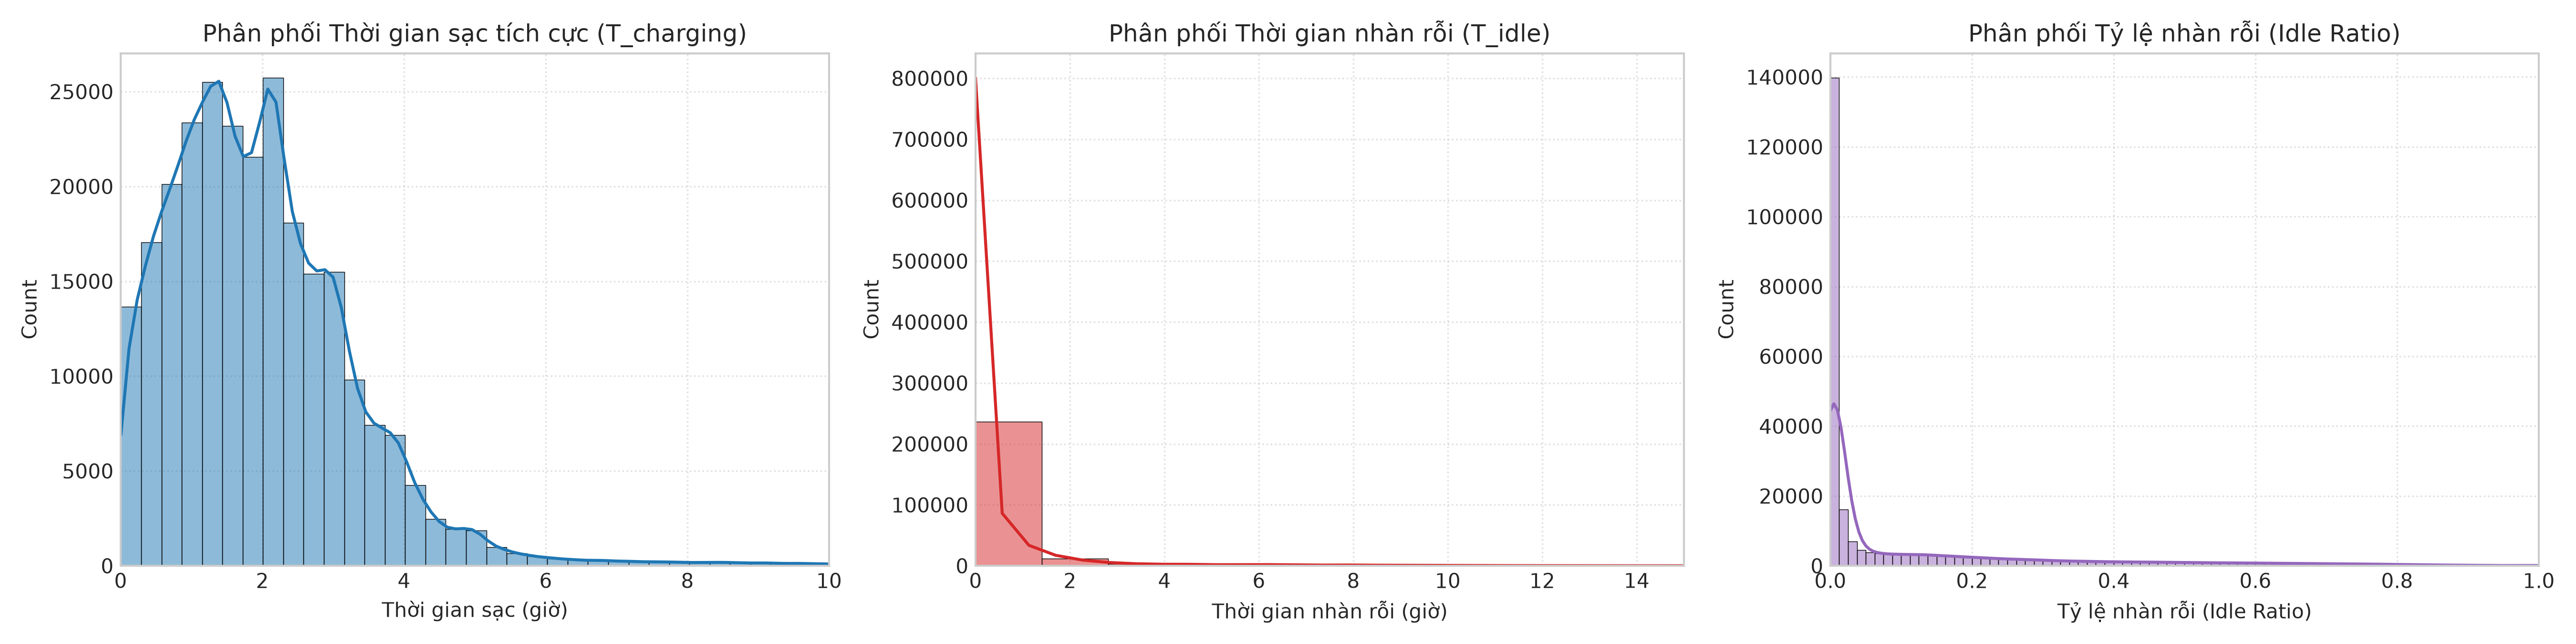
\includegraphics[width=\columnwidth]{feature_distributions_occupancy.png}
\caption{Phân phối thời gian sạc,
thời gian nhàn rỗi và tỷ lệ nhàn rỗi.}
\label{fig:eda_idle}
\end{figure}

Bên cạnh các đặc trưng về thời lượng,
dữ liệu còn được tổng hợp theo
giờ bắt đầu phiên, ngày trong tuần
và năm để khảo sát
xu hướng nhu cầu sử dụng.

Kết quả EDA cho thấy
11 giờ là thời điểm có
số phiên bắt đầu cao nhất,
với 21.015 phiên
(8,12\% tập phân tích).
Ngược lại, 2 giờ sáng
có 128 phiên (0,05\%).

Số phiên theo năm cũng biến động
đáng kể trong giai đoạn quan sát.
Năm 2017 ghi nhận 48.857 phiên,
trong khi năm 2020
giảm còn 20.064 phiên.
Diễn biến năm 2020 cần được
xem xét trong bối cảnh đại dịch
COVID-19 và không nên
quy toàn bộ thay đổi nhu cầu
cho chính sách giá.

% ==========================================
% HÌNH III.2
% Dùng biểu đồ số phiên sạc theo năm
% trong phần EDA của báo cáo gốc.
% ==========================================

\begin{figure}[!t]
\centering
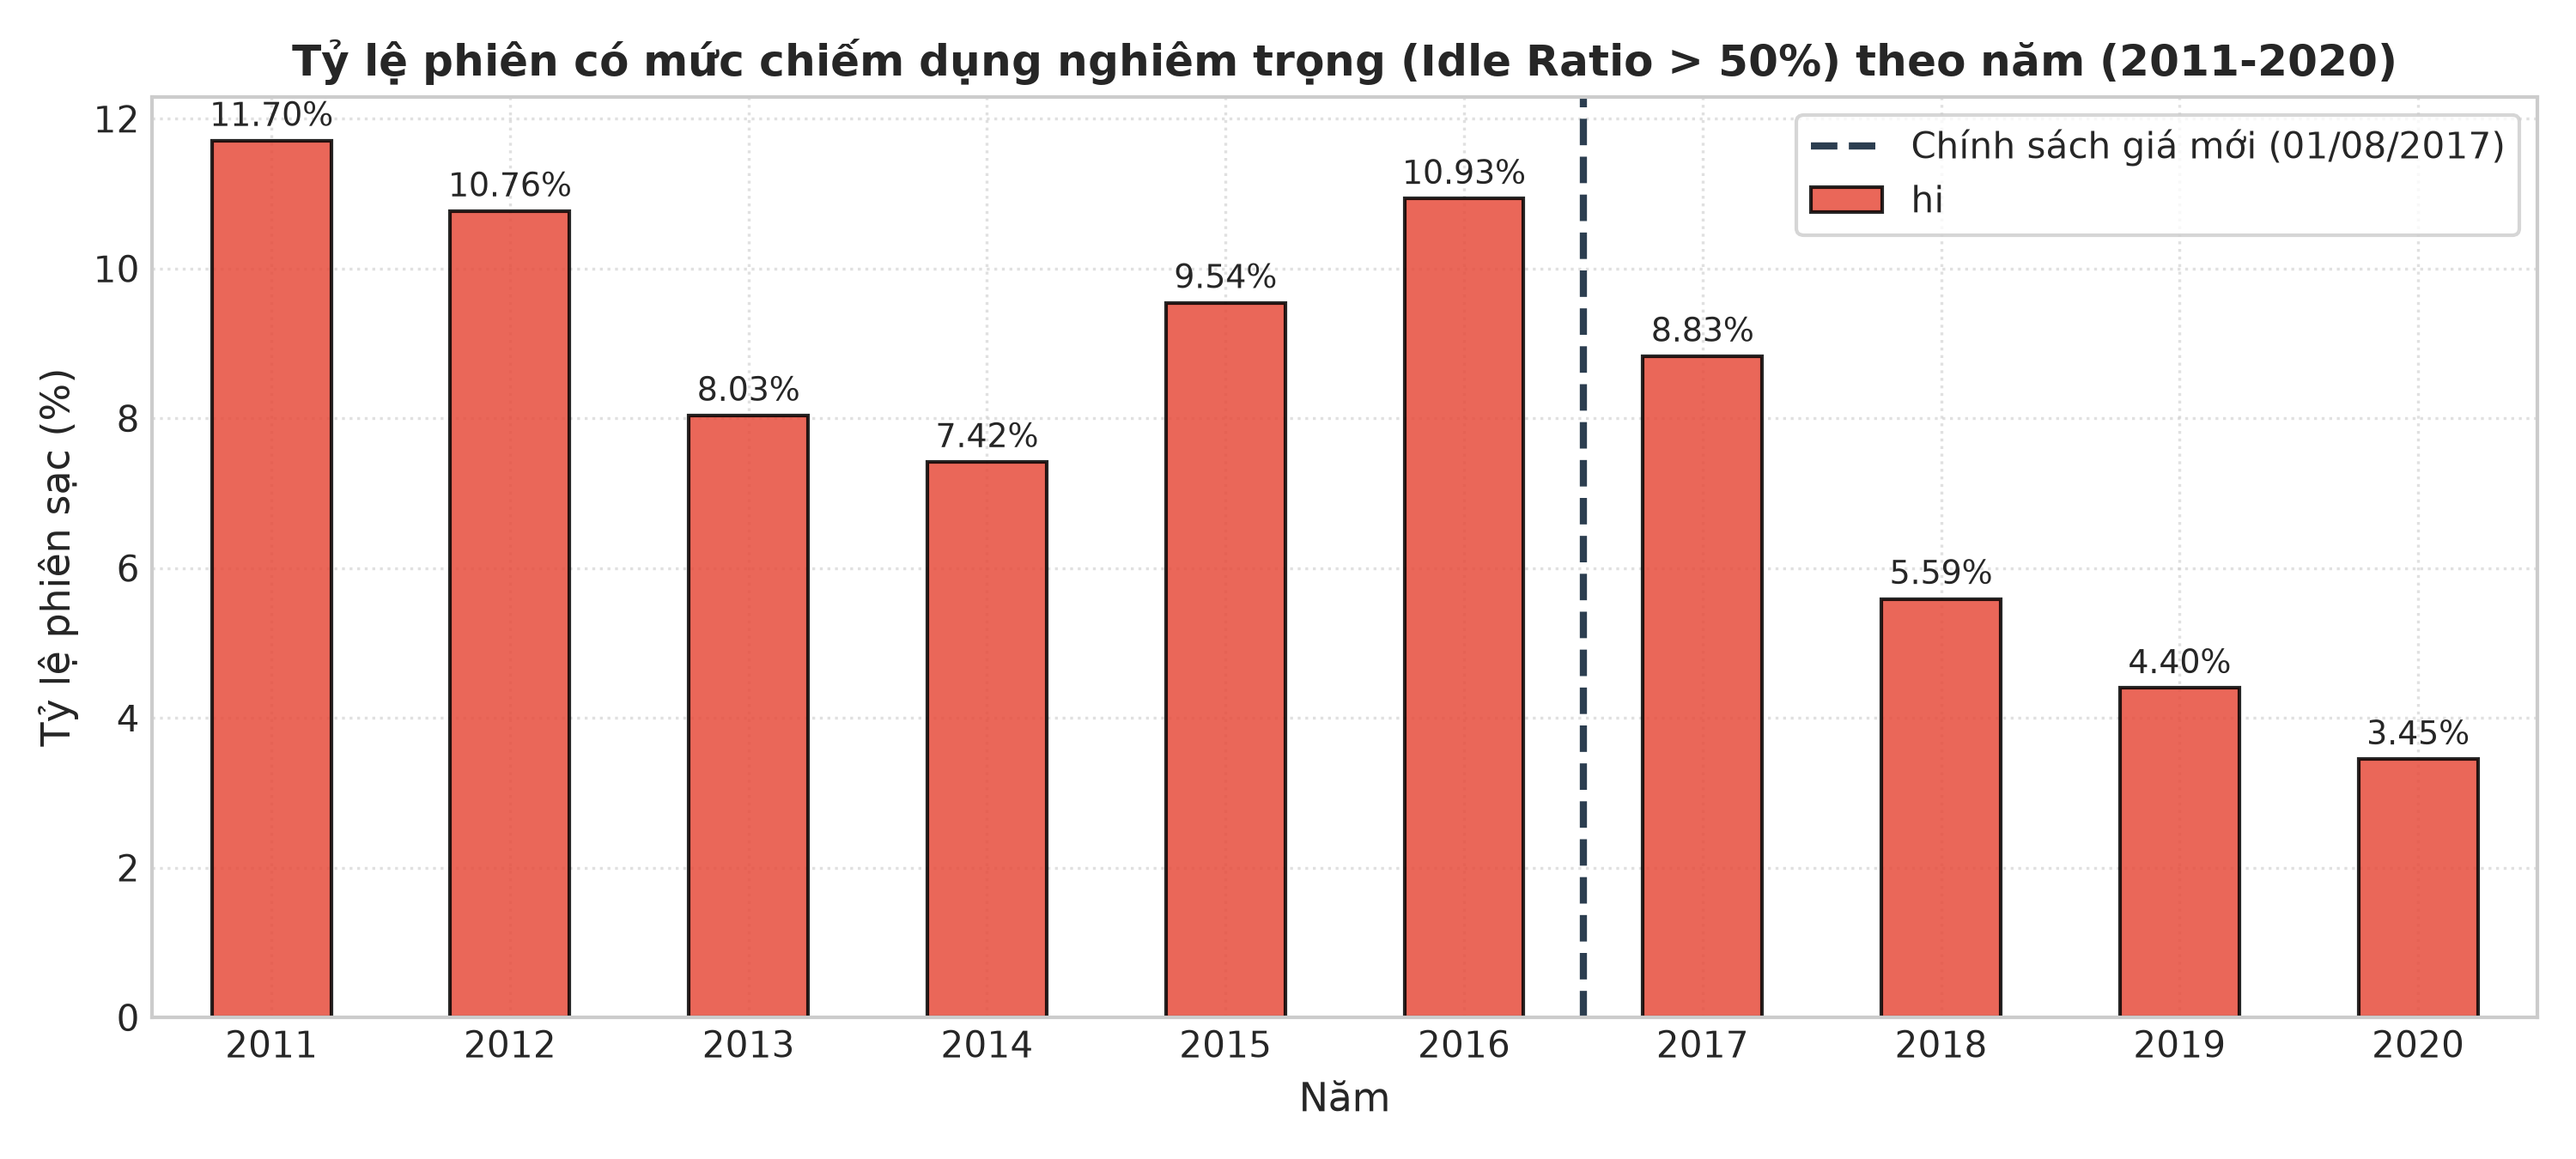
\includegraphics[width=\columnwidth]{yearly_high_idle_ratio_trend.png}
\caption{Tỷ lệ phiên có Idle Ratio trên 50\%
theo năm trong giai đoạn 2011--2020.}
\label{fig:sessions_year}
\end{figure}

\subsection{Dữ liệu phục vụ các nhiệm vụ
phân tích tiếp theo}

Các nhiệm vụ NV2--NV5
sử dụng những tập dữ liệu
được xác định theo
điều kiện riêng của từng bài toán.

NV2 thực hiện phân cụm trên
258.720 phiên sau các bước
loại trùng, kiểm tra logic,
lọc công suất theo ngưỡng
19,2 kW của thí nghiệm
và đối chiếu timestamp.

NV3 sử dụng dữ liệu cấp phiên
và định danh người dùng
để so sánh hành vi
trước và sau ngày 01/08/2017.

NV4 tổng hợp dữ liệu theo trạm
để xây dựng ma trận
sáu tiêu chí vận hành.
Các trạm không đạt
ngưỡng tối thiểu 500 phiên
không được đưa vào xếp hạng,
còn 33 trạm đủ điều kiện.

NV5 sử dụng các phiên hợp lệ
được xử lý theo quy tắc riêng
để xây dựng chuỗi thời gian
15 phút theo cụm vị trí,
phục vụ dự báo số phiên mới
và số cổng bị chiếm dụng.

Do các nhiệm vụ có
đơn vị phân tích,
điều kiện lọc và mục tiêu
khác nhau, kích thước mẫu
không nhất thiết giống nhau.

Việc ghi nhận rõ
quy mô và điều kiện lựa chọn
ở từng nhiệm vụ giúp
bảo đảm tính nhất quán
khi diễn giải kết quả thực nghiệm.

% ==========================================


% ==========================================
% TÀI LIỆU THAM KHẢO CHUẨN IEEE
% Mở rộng khi viết các phần III-VII
% ==========================================

\begin{thebibliography}{00}

\bibitem{bayram2023}
I. S. Bayram, A. Saad, R. Sims,
A. Babu, C. Edmunds, and S. Galloway,
``Statistical Characterization of
Public AC EV Chargers in the U.K.,''
\textit{IEEE Access},
vol. 11, 2023,
doi: 10.1109/ACCESS.2023.3293091.

\bibitem{straka2019}
M. Straka and L. Buzna,
``Clustering algorithms applied
to usage related segments of
electric vehicle charging stations,''
\textit{Transportation Research Procedia},
vol. 40, pp. 1576--1582, 2019,
doi: 10.1016/j.trpro.2019.07.218.

\bibitem{luowang2025}
S. Luo and Y. Wang,
``The impacts of rate surge on
electric vehicle charging behaviors:
Evidence from California,''
\textit{Journal of Economic Behavior
\& Organization},
vol. 236, Art. no. 107048, 2025,
doi: 10.1016/j.jebo.2025.107048.

\bibitem{ostermann2022}
A. Ostermann, Y. Fabel,
K. Ouan, and H. Koo,
``Forecasting Charging Point Occupancy
Using Supervised Learning Algorithms,''
\textit{Energies},
vol. 15, no. 9, Art. no. 3409, 2022,
doi: 10.3390/en15093409.

\end{thebibliography}

\end{document}
